% ---------------------------------------------------------------------
% -------------- PREAMBLE ---------------------------------------------
% ---------------------------------------------------------------------
\documentclass[12pt,a4paper,finnish,oneside]{article}
%\documentclass[12pt,a4paper,finnish,twoside]{article}
%\documentclass[12pt,a4paper,finnish,oneside,draft]{article} % luonnos, nopeampi

% Valitse 'input encoding':
%\usepackage[latin1]{inputenc} % merkistökoodaus, jos ISO-LATIN-1:tä.
\usepackage[utf8x]{inputenc}   % merkistökoodaus, jos käytetään UTF8:a
%\usepackage[utf8]{luainputenc}
% Valitse 'output/font encoding':
\usepackage[T1]{fontenc}      % korjaa ääkkösten tavutusta, bittikarttana
%\usepackage{ae,aecompl}       % ed. lis. vektorigrafiikkana bittikartan sijasta
% Kieli- ja tavutuspaketit:
\usepackage[english,swedish,finnish]{babel}
% Kurssin omat asetukset aaltosci_t.sty:
%\usepackage{aaltosci_t}
% Jos kirjoitat muulla kuin suomen kielellä valitse:
%\usepackage[finnish]{aaltosci_t}           
\usepackage[swedish]{aaltosci_t}           
%\usepackage[english]{aaltosci_t}           
% Muita paketteja:
\usepackage{alltt}
\usepackage{amsmath}   % matematiikkaa
\usepackage{calc}      % käytetään laskurien (counter) yhteydessä (tiedot.tex)
\usepackage{eurosym}   % eurosymboli: \euro{}
\usepackage[obeyspaces]{url}       % \url{...}
\usepackage{listings}  % koodilistausten lisääminen
\usepackage{algorithm} % algoritmien lisääminen kelluvina
\usepackage{algorithmic} % algoritmilistaus
\usepackage{hyphenat}  % tavutuksen viilaamiseen liittyvä (hyphenpenalty,...)
\usepackage{supertabular,array}  % useampisivuinen taulukko
\usepackage{hyperref}
\usepackage{graphicx}

% Koko dokumentin kattavia asetuksia:

% Tavutettavia sanoja:
%\hyphenation{vää-rin me-ne-vi-en eri-kois-ten sa-no-jen tavu-raja-ehdo-tuk-set}
% Huomaa, että ylläoleva etsii tarkalleen kyseisiä merkkijonoja, eikä
% ymmärrä taivutuksia. Paikallisesti tekstin seassa voi myös ta\-vut\-taa.

% Rangaistaan tavutusta (ei toimi?! Onko hyphenat-paketti asennettu?)
\hyphenpenalty=10000   % rangaistaan tavutuksesta, 10000=ääretön
\tolerance=1000        % siedetään välejä riveillä
% titlesec-paketti auttaa, jos tämän mukana menee sekaisin

% Tekstiviitteiden ulkoasu.
% Pakettiin natbib.sty/aaltosci.bst liittyen katso esim. 
% http://merkel.zoneo.net/Latex/natbib.php
% jossa selitykset citep, citet, bibpunct, jne.
% Valitse alla olevista tai muokkaa:
%\bibpunct{(}{)}{;}{a}{,}{,}    % a = tekijä-vuosi (author-year)
\bibpunct{[}{]}{;}{n}{,}{,}    % n = numero [1],[2] (numerical style)

% Rivivälin muuttaminen:
\linespread{1.24}\selectfont               % riviväli 1.5
%\linespread{1.24}\selectfont               % riviväli 1, kun kommentoit pois

% ---------------------------------------------------------------------
% -------------- DOCUMENT ---------------------------------------------
% ---------------------------------------------------------------------

\begin{document}

% -------------- Tähän dokumenttiin liittyviä valintoja  --------------

%\raggedright         % Tasattu vain vasemmalta, ei tavutusta
% ----------------- joitakin makroja ----------------------------------
%
% \newcommand{\sinunKomentosi}[argumenttienMäärä]{komennot%
% voiJakaaRiveille%
% jaArgumenttienViittaus#1,#2,#argumenttienMäärä}

% Joskus voi olla tarpeen kommentoida jotakin. Ei suositella. 
% Äläkä unohda lopulliseen! 
\newcommand{\Kommentti}[1]{\fbox{\textbf{OMA KOMMENTTI:} #1}}
% Käyttö: Kilometri on 1024 metriä. \Kommentti{varmista tämä vielä}.
% Eli newcommand:n komentosanan jälkeen hakasaluissa argumenttien lkm,
%  ja argumentteihin viitataa #1, #2, ...

%  Comment out this \DRAFT macro if this version no longer is one!  XXX
%\newcommand{\DRAFT}{\begin{center} {\it DRAFT! \hfill --- \hfill DRAFT!
%\hfill --- \hfill DRAFT! \hfill --- \hfill DRAFT!}\end{center}}

%  Use this \DRAFT macro in the final version - or comment out the 
%  draft-command
% \newcommand{\DRAFT}{~}

% %%%%%%%% MATEMATIIKKA %%%%%%%%%%%%%%%%%

% Määrätty integraali
\newcommand{\myInt}[4]{%
\int_{#1}^{#2} #3 \, \textrm{d}{#4}}

% http://kapsi.fi/jks/satfaq/
%\newcommand{\vii}{\mathop{\Big/}}
%\newcommand{\viiva}[2]{\vii\limits_{\!\!\!\!{#1}}^{\>\,{#2}}}
%%\[ \intop_0^{10} \frac{x}{x^2+1} \,\mathrm{d}x
%%= \viiva{0}{10} \frac{1}{2}\ln(x^2+1) \]

% matht.sty, Simo K. Kivelä, 01.01.2002, 07.04.2004, 19.11.2004, 21.02.2005
% Kokoelma matemaattisten lausekkeiden kirjoittamista helpottavia
% määrittelyjä.

% 07.04.2004 Muutama lisäys ja muutos tehty: \ii, \ee, \dd, \der,
% \norm, \abs, \tr.
%
% 19.11.2004 Korjattu määrittelyjä: \re, \im, \norm;
% lisätty \trp (transponointi), \hrm (hermitointi), \itgr (rakenteellinen
% integraali), ympäristö Cmatrix (hakasulkumatriisi);
% vanha transponointi \tr on mukana edelleen, mutta ei suositella.

% Pakotettu rivinvaihto, joka voidaan tarvittaessa määritellä
% uudelleen: 

%\newcommand{\nl}{\newline}

% Logiikan symboleja (<=> ja =>) hieman muunnettuina:

%\newcommand{\ifftmp}{\;\Leftrightarrow\;}
%\newcommand{\impltmp}{\DOTSB\;\Rightarrow\;}

% 'siten, että' -lyhenne ja hattupääyhtäläisyysmerkki vastaavuuden
% osoittamiseen: 

%\newcommand{\se}{\quad \text{siten, että} \quad}
%\newcommand{\vs}{\ {\widehat =}\ }

% Lukujoukkosymbolit:

%\newcommand{\N}{\ensuremath{\mathbb N}}
%\newcommand{\Z}{\ensuremath{\mathbb Z}}
%\newcommand{\Q}{\ensuremath{\mathbb Q}}
%\newcommand{\R}{\ensuremath{\mathbb R}}
%\newcommand{\C}{\ensuremath{\mathbb C}}

% Reaali- ja imaginaariosa, imaginaariyksikkö:

%\newcommand{\re}{\operatorname{Re}}
%\newcommand{\im}{\operatorname{Im}}
%\newcommand{\ii}{\mathrm{i}}

% Differentiaalin d, Neperin luku:

%\newcommand{\dd}{\mathrm{d}}
%\newcommand{\ee}{\mathrm{e}}

% Vektorimerkintä, joka voidaan tarvittaessa määritellä uudelleen
% (tämä tekee vektorit lihavoituina):

%\newcommand{\V}[1]{{\mathbf #1}}

% Kulmasymboli:

%\renewcommand{\angle}{\sphericalangle}

% Vektorimerkintä, jossa päälle pannaan iso nuoli;
% esimerkiksi \overrightarrow{AB} (tämmöisiä olemassaolevien
% symbolien uudelleenmäärittelyjä ei kyllä pitäisi tehdä):

%\renewcommand{\vec}[1]{\overrightarrow{#1}}

% Vektoreiden vastakkaissuuntaisuus:

%\newcommand{\updownarrows}{\uparrow\negthinspace\downarrow}

% Itseisarvot ja normi:

%\newcommand{\abs}[1]{{\left\vert#1\right\vert}}
%\newcommand{\norm}[1]{{\left\Vert #1 \right\Vert}}

% Transponointi ja hermitointi:

%\newcommand{\trp}[1]{{#1}\sp{\operatorname{T}}}
%\newcommand{\hrm}[1]{{#1}\sp{\operatorname{H}}}

% Vanha transponointi; jäljellä yhteensopivuussyistä, ei syytä käyttää.
%\newcommand{\tr}{{}^{\text T}}

% Arcus- ja area-funktiot, jossa päähaara osoitetaan nimen päälle
% vedetyllä vaakasuoralla viivalla (alkaa olla vanhentunutta,
% voitaisiin luopua):

%\newcommand{\arccot}{\operatorname{arccot}}
%\newcommand{\asin}{\operatorname{\overline{arc}sin}}
%\newcommand{\acos}{\operatorname{\overline{arc}cos}}
%\newcommand{\atan}{\operatorname{\overline{arc}tan}}
%\newcommand{\acot}{\operatorname{\overline{arc}cot}}

%\newcommand{\arsinh}{\operatorname{arsinh}}
%\newcommand{\arcosh}{\operatorname{arcosh}}
%\newcommand{\artanh}{\operatorname{artanh}}
%\newcommand{\arcoth}{\operatorname{arcoth}}
%\newcommand{\acosh}{\operatorname{\overline{ar}cosh}}

% Signum, syt, pyj:

%\newcommand{\sg}{\operatorname{sgn}}
%\renewcommand{\gcd}{\operatorname{syt}}
%\newcommand{\lcm}{\operatorname{pyj}}

% Lyhennemerkintöjä: derivaatta, osittaisderivaatta, gradientti,
% derivaattaoperaattori, vektorin komponentti, integraalin ylä- ja
% alasumma, Suomessa (ja Saksassa?) käytetty integraalin sijoitus-
% merkintä, integraali (rakenteellinen määrittely):

%\newcommand{\der}[2]{\frac{\dd #1}{\dd #2}}
%\newcommand{\osder}[2]{\frac{\partial #1}{\partial #2}}
%\newcommand{\grad}{\operatorname{grad}}
%\newcommand{\Df}{\operatorname{D}} 
%\newcommand{\comp}{\operatorname{comp}}
%\newcommand{\ys}[1]{\overline S_{#1}}
%\newcommand{\as}[1]{\underline S_{#1}}
%\newcommand{\sijoitus}[2]{\biggl/_{\null\hskip-6pt #1}^{\null\hskip2pt #2}} 
%\newcommand{\itgr}[4]{\int_{#1}^{#2}#3\,\dd #4}

% Matriiseja, joille voidaan antaa alkioiden sijoittamista sarakkeen
% vasempaan tai oikeaan reunaan tai keskelle osoittava lisäparametri
% (l, r tai c); ympärillä kaarisulut, hakasulut, pystyviivat (determinantti)
% tai ei mitään;
% esimerkiksi \begin{cmatrix}{ll}1 & -1 \\ -1 & 1 \end{cmatrix}:

%\newenvironment{cmatrix}[1]{\left(\begin{array}{#1}}{\end{array}\right)}
%\newenvironment{Cmatrix}[1]{\left[\begin{array}{#1}}{\end{array}\right]}
%\newenvironment{dmatrix}[1]{\left|\begin{array}{#1}}{\end{array}\right|}
%\newenvironment{ematrix}[1]{\begin{array}{#1}}{\end{array}}

% Kaunokirjoitussymboli:

%\newcommand{\Cal}{\mathcal}

% Isokokoinen summa:

%\newcommand{\dsum}[2]{{\displaystyle \sum_{#1}^{#2}}}

% Tuplaintegraali umpinaisen pinnan yli; korvataan jos parempi löytyy:
%\newcommand\oiint{\begingroup
% \displaystyle \unitlength 1pt
% \int\mkern-7.2mu
% \begin{picture}(0,3)
%   \put(0,3){\oval(10,8)}
% \end{picture}
% \mkern-7mu\int\endgroup}
       % Haetaan joitakin makroja

% Kieli:
% Kielesi, jolla kandidaatintyön kirjoitat: finnish, swedish, english.
% Tästä tulee mm. tietyt otsikkonimet ja kuva- ja taulukkoteksteihin 
% (Kuva, Figur, Figure), (Taulukko, Tabell, Table) sekä oikea tavutus.
%\selectlanguage{finnish}
\selectlanguage{swedish}
%\selectlanguage{english}

% Sivunumeroinnin kanssa pieniä ristiriitaisuuksia.
% Toimitaan pääosin lähteen "Kirjoitusopas" luvun 5.2.2 mukaisesti.
% Sivut numeroidaan juoksevasti arabialaisin siten että 
% ensimmäiseltä nimiölehdeltä puuttuu numerointi.
\pagestyle{plain}
\pagenumbering{arabic}
% Muita tapoja: kandiohjeet: ei numerointia lainkaan ennen tekstiosaa
%\pagestyle{empty}
% Muita tapoja: kandiohjeet: roomalainen numerointi alussa ennen tekstiosaa
%\pagestyle{plain}
%\pagenumbering{roman}        % i,ii,iii, samalla alustaa laskurin ykköseksi

% ---------------------------------------------------------------------
% -------------- Luettelosivut alkavat --------------------------------
% ---------------------------------------------------------------------

% -------------- Nimiölehti ja sen tiedot -----------------------------
%
% Nimiölehti ja tiivistelmä kirjoitetaan seminaarin mukaan joko
% suomeksi tai ruotsiksi (ellei erityisesti kielenä ole englanti). 
% Tiivistelmän voi suomen/ruotsin lisäksi kirjoittaa halutessaan
% myös englanniksi. Eli tiivistelmiä tulee yksi tai kaksi kpl.
%
% "\MUUTTUJA"-kohdat luetaan aaltosci_t.sty:ä varten.

\author{Jonathan Rehn}

% Otsikko nimiölehdelle. Yleensä sama kuin seuraavana oleva \TITLE, 
% mutta jos nimiölehdellä tarvetta "kaksiosaiselle" kaksiriviselle
\title{Jämförelse av ramverk för uppskalning av agil utveckling}
% 2-osainen otsikko:
%\title{\LaTeX{}-pohja kandidaatintyölle \\[5mm] Pitkiä rivejä kokeilun vuoksi.}

% Otsikko tiivistelmään. Jos lisäksi engl. tiivistelmä, niin viimeisin:
\TITLE{Jämförelse av ramverk för uppskalning av agil utveckling}
%\TITLE{\LaTeX{} för kandidatseminariet med jättelång rubrik som fortsätter och
% fortsätter ännu}
\ENTITLE{\LaTeX{} template for Bachelor thesis with a pretty long title %
line which continues ynd continues}
% 2-osainen otsikko korvataan täällä esim. pisteellä:
%\TITLE{\LaTeX{}-pohja kandidaatintyölle. Pitkiä rivejä kokeilun vuoksi.}

% Ohjaajan laitos suomi/ruotsi ja tarvittaessa eng (tiivistelmän kieli/kielet)
%\DEPT{Poimi tähän ohjaajasi laitos, DEPT, main.tex}
% suomi:
%\DEPT{Tietotekniikan laitos}               % T
%\DEPT{Tietojenkäsittelytieteen laitos}     % TKT
%\DEPT{Mediatekniikan laitos}               % ME
% ruotsi:
\DEPT{Institutionen för datateknik}        % T
%\DEPT{Institutionen för datavetenskap}     % TKT
%\DEPT{Institutionen för mediateknik}       % ME
% englanti:
%\ENDEPT{Department of Computer Science Engineering}     % T
%\ENDEPT{Department of Information and Computer Science} % TKT
%\ENDEPT{Department of Media Technology}                 % ME

% Vuosi ja päivämäärä, jolloin työ on jätetty tarkistettavaksi.
\YEAR{2016}
%\DATE{xx. xxxxxkuuta 20xx}
%\DATE{31. helmikuuta 2011}
\DATE{Den 27 juli 2016}
\ENDATE{July 27, 2016}

% Kurssin vastuuopettaja ja työsi ohjaaja(t)
\SUPERVISOR{Prof. Juho Rousu}
\INSTRUCTOR{TkD Maria Paasivaara}
%\INSTRUCTOR{Ohjaajantitteli Sinun Ohjaajasi, ToinenTitt Matti Meikäläinen}
% DI       // på svenska DI diplomingenjör
% TkL      // TkL teknologie licentiat
% TkT      // TkD teknologie doctor
% Dosentti Dos. // Doc. Docent
% Professori Prof. // Prof. Professor
% 
% Jos tiivistelmä englanniksi, niin:
\ENSUPERVISOR{TitleOfResponsibleTeacher NameofResponsibleTeacher}
\ENINSTRUCTOR{Maria Paasivaara, TkD}
% M.Sc. (Tech)  // M.Sc. (Eng)
% Lic.Sc. (Tech)
% D.Sc. (Tech)   // FT filosofian tohtori, PhD Doctor of Philosophy
% Docent
% Professor

% Kirjoita tänne HOPS:ssa vahvistettu pääaineesi.
% Pääainekoodit TIK-opinto-oppaasta.

\PAAAINE{Datateknik}
\CODE{SCI3027}

%\PAAAINE{Ohjelmistotuotanto ja -liiketoiminta}
%\CODE{T3003}
%
%\PAAAINE{Tietoliikenneohjelmistot}
%\CODE{T3005}
%
%\PAAAINE{WWW-teknologiat} % vuodesta 2010
%\CODE{IL3012}
%
%\PAAAINE{Mediatekniikka} % vuoteen 2010, kts. seur.
%\CODE{T3004}
%
%\PAAAINE{Mediatekniikka} % vuodesta 2010, kts. edell.
%\CODE{IL3011}
%
%\PAAAINE{Tietojenkäsittelytiede} % vuodesta 2010
%\CODE{IL3010}
%
%\PAAAINE{Informaatiotekniikka} % vuoteen 2010
%\CODE{T3006}
%
%\PAAAINE{Tietojenkäsittelyteoria} % vuoteen 2010
%\CODE{T3002}
%
%\PAAAINE{Ohjelmistotekniikka}
%\CODE{T3001}

% Avainsanat tiivistelmään. Tarvittaessa myös englanniksi:

\KEYWORDS{agile, scrum, scaling, frameworks}
\ENKEYWORDS{key, words, the same as in FIN/SWE}

% Tiivistelmään tulee opinnäytteen sivumäärä.
% Kirjoita lopulliset sivumäärät käsin tai kokeile koodia. 
%
% Ohje 29.8.2011 kirjaston henkilökunnalta:
%   - yhteissivumäärä nimiölehdeltä ihan loppuun
%   - "kaikkien yksinkertaisin ja yksiselitteisin tapa"
%
% VANHA // Ohje 14.11.2006, luku 4.2.5:
% VANHA // - sivumäärä = tekstiosan (alkaen johdantoluvusta) ja 
% VANHA //  lähdeluettelon sivumäärä, esim. "20"
% VANHA // - jos liitteet, niin edellisen lisäksi liitteiden sivumäärä,
% VANHA //  tyyli "20 + 5", jossa 5 sivua liitteitä 
% VANHA // - HUOM! Tässä oletuksena sivunumerointi alkaa nimiölehdestä 
% VANHA //  sivunumerolla 1. %   Toisin sanoen, viimeisen lähdeluettelosivun 
% VANHA //  sivunumero EI ole sivujen määrä vaan se pitää laskea tähän käsin

\PAGES{8}
%\PAGES{23}  % kaikki sivut laskettuna nimiölehdestä lähdeluettelon tai 
             % mahdollisten liitteiden loppuun. Tässä 23 sivua

%\thispagestyle{empty}  % nimiölehdellä ei ole sivunumerointia; tyylin mukaan ei tehdäkään?!

\maketitle             % tehdään nimiölehti

% -------------- Tiivistelmä / abstract -------------------------------
% Lisää abstrakti kandikielellä (ja halutessasi lisäksi englanniksi).

% Edelleen sivunumerointiin. Eräs ohje käskee aloittaa sivunumeroiden
% laskemisen nimiösivulta kuitenkin niin, että sille ei numeroa merkitä
% (Kauranen, luku 5.2.2). Näin ollen ensimmäisen tiivistelmän sivunumero
% on 2. \maketitle komento jotenkin kadottaa sivunumeronsa.
\setcounter{page}{2}    % sivunumeroksi tulee 2

% Tiivistelmät tehdään viimeiseksi. 
%
% Tiivistelmä kirjoitetaan käytetyllä kielellä (JOKO suomi TAI ruotsi)
% ja HALUTESSASI myös samansisältöisenä englanniksi.
%
% Avainsanojen lista pitää merkitä main.tex-tiedoston kohtaan \KEYWORDS.

\begin{fiabstract}
  Tiivistelmä on muusta työstä täysin irrallinen teksti, joka
  kirjoitetaan tiivistelmälomakkeelle vasta, kun koko työ on
  valmis. Se on suppea ja itsenäinen teksti, joka kuvaa olennaisen
  opinnäytteen sisällöstä. Tavoitteena selvittää työn merkitys
  lukijalle ja antaa yleiskuva työstä. Tiivistelmä markkinoi työtäsi
  potentiaalisille lukijoille, siksi tutkimusongelman ja tärkeimmät
  tulokset kannattaa kertoa selkeästi ja napakasti. Tiivistelmä
  kirjoitetaan hieman yleistajuisemmin kuin itse työ, koska teksti
  palvelee tiedonvälitystarkoituksessa laajaa yleisöä.

  Tiivistelmän rakenne: 
teksti jäsennetään kappaleisiin (3--5 kappaletta);
ei väliotsikkoja; 
ei mitään työn ulkopuolelta; 
ei tekstiviitteitä tai lainauksia;
vähän tai ei ollenkaan viittauksia työhön 
(ei ollenkaan: ``luvussa 3'' tms., mutta koko työhön voi 
viitata esim. sanalla ``kandidaatintyössä'';
ei kuvia ja taulukoita.

Tiivistelmässä otetaan ``löysät pois'':
ei työn rakenteen esittelyä;
ei itsestäänselvyyksiä;
ei turhaa toistoa;
älä jätä lukijaa nälkäiseksi, eli kerro asiasisältö, 
älä vihjaa, että työssä kerrotaan se.

Tiivistelmän tyypillinen rakenne: 
(1) aihe, tavoite ja rajaus 
(heti alkuun, selkeästi ja napakasti, ei johdattelua);
(2) aineisto ja menetelmät (erittäin lyhyesti);
(3) tulokset (tälle enemmän painoarvoa); 
(4) johtopäätökset (tälle enemmän painoarvoa).
%
%Tiivistelmätekstiä tähän (\languagename). Huomaa, että tiivistelmä tehdään %vasta kun koko työ on muuten kirjoitettu.
\end{fiabstract}

%\begin{svabstract}
%  Ett abstrakt hit 
%%(\languagename)
%\end{svabstract}

%\begin{enabstract}
% Here goes the abstract 
%%(\languagename)
%\end{enabstract}

\newpage                       % pakota sivunvaihto

% -------------- Sisällysluettelo / TOC -------------------------------

\tableofcontents

%\label{pages:prelude}
%\clearpage                     % kappale loppuu, loput kelluvat tänne, sivunv.
%\newpage

% -------------- Symboli- ja lyhenneluettelo -------------------------
% Lyhenteet, termit ja symbolit.
% Suositus: Käytä vasta kun paljon symboleja tai lyhenteitä.
%
%% -------------- Symbolit ja lyhenteet --------------
%
% Suomen kielen lehtorin suositus: vasta kun noin 10-20 symbolia
% tai lyhennettä, niin käytä vasta sitten.
%
% Tämä voi puuttuakin. Toisaalta jos käytät paljon akronyymejä,
% niin ne kannattaa esitellä ensimmäisen kerran niitä käytettäessä.
% Muissa tapauksissa lukija voi helposti tarkistaa sen tästä
% luettelosta. Esim. "Automaattinen tietojenkäsittely (ATK) mahdollistaa..."
% "... ATK on ..."

\addcontentsline{toc}{section}{Käytetyt symbolit ja lyhenteet}

\section*{Använda symboler och förkortningar}
%?? Käytetyt lyhenteet ja termit ??
%?? Käytetyt lyhenteet / termit / symbolit ??
%\section*{Abbreviations and Acronyms}

\begin{center}
\begin{tabular}{p{0.2\textwidth}p{0.65\textwidth}}

DAD & Discipilined Agile Delivery \\ 
SAFe & Scaled Agile Framework \\ 
LeSS & Large Scale Scrum \\

\end{tabular}
\end{center}

\vspace{10mm}

%Jos tarvitset useampisivuista taulukkoa, kannattanee käyttää 
%esim. \verb!supertabular*!-ympäristöä, josta on kommentoitu esimerkki
%toisaalla tekstiä.


 
%\clearpage                     % luku loppuu, loput kelluvat tänne
\newpage

% -------------- Kuvat ja taulukot ------------------------------------
% Kirjoissa (väitöskirja) on usein tässä kuvien ja taulukoiden listaus.
% Suositus: Ei kandityöhön.

% -------------- Alkusanat --------------------------------------------
% Suositus: ÄLÄ käytä kandidaatintyössä. Jos käytät, niin omalle 
% sivulleen käyttäen tarvittaessa \newpage
%
%% --------------- Alkusanat -------------------------------------------
%
% Suositus: Älä käytä kandidaatintyössä.
%

\addcontentsline{toc}{section}{Alkusanat}

\section*{Alkusanat}
%\section*{Förord}
%\section*{Acknowledgements}

Alkusanoissa voi kiittää tahoja, jotka ovat merkittävästi edistäneet
työn valmistumista. Tällaisia voivat olla esimerkiksi yritys, jonka
tietokantoja, kontakteja tai välineistöä olet saanut käyttöösi,
haastatellut henkilöt, ohjaajasi tai muut opettajat ja myös
henkilökohtaiset kontaktisi, joiden tuki on ollut korvaamatonta työn
kirjoitusvaiheessa. Alkusanat jätetään tyypillisesti pois
kandidaatintyöstä, joka on laajuudeltaan vielä niin suppea, ettei
kiiteltäviä tahoja luontevasti ole.

\textbf{TIK.kand suositus: Älä käytä tällaista lukua.}

\vskip 10mm
Espoossa 31. helmikuuta 2011
\vskip 15mm
Teemu Teekkari


%\clearpage                     % luku loppuu, loput kelluvat tänne
%\newpage                       % pakota sivunvaihto
%
%SH: Alkusanoissa voi kiittää tahoja, jotka ovat merkittävästi edistäneet
% työn valmistumista. Tällaisia voivat olla esimerkiksi yritys, jonka
% tietokantoja, kontakteja tai välineistöä olet saanut käyttöösi,
% haastatellut henkilöt, ohjaajasi tai muut opettajat ja myös
% henkilökohtaiset kontaktisi, joiden tuki on ollut korvaamatonta työn
% kirjoitusvaiheessa. Alkusanat jätetään tyypillisesti pois
% kandidaatintyöstä, joka on laajuudeltaan vielä niin suppea, ettei
% kiiteltäviä tahoja luontevasti ole.

% ---------------------------------------------------------------------
% -------------- Tekstiosa alkaa --------------------------------------
% ---------------------------------------------------------------------

% Muutetaan tarvittaessa ala- ja ylätunnisteet
%\pagestyle{headings}          % headeriin lisätietoja
%\pagestyle{fancyheadings}     % headeriin lisätietoja
%\pagestyle{plain}             % ei header, footer: sivunumero

% Sivunumerointi, jos käytetty 'roman' aiemmin
% \pagenumbering{arabic}        % 1,2,3, samalla alustaa laskurin ykköseksi
% \thispagestyle{empty}         % pyydetty ensimmäinen tekstisivu tyhjäksi

% input-komento upottaa tiedoston 
\section{Inledning}
	
	%Vadå ramverk för agil uppskalning
	Detta arbete jämför olika ramverk för uppskalning av agil programutveckling. Dessa ger metoder och principer för att applicera mer traditionella agila metoder på större projekt och grupper.
	
	%agila metoder
	Agil programutveckling är i sig ett iterativt och inkrementellt sätt att utveckla programvara.
	
	%meta
	Detta arbete är indelat i fyra huvudkapitel. Inledningen utgör i sin helhet det första kapitilet.
	I andra kapitlet behandlas bakgrunden till själva frågeställningen. Tekniska definitioner för Agil utveckling, dess skalning samt de olika ramverken för det presenteras. 
	Det tredje kapitlet formulerar syftet med arbetet samt ämnets avgränsningar. Materialet och vilka metoder som används presenteras även i tredje kapitlet.
	
	Sista kapitlet behandlar själva reslutatet av arbetet och vilka slutsatser som dras av det.
	
\newpage
\section{Bakgrund} 	
	
	%TODO: Teoretisk bakgrund och genomgång av problemuppläggningen
	
	I detta stycke behandlas den tekniska bakgrunden till arbetet. Central bakgrundskunskap förutsatt av läsaren presenteras här.
	
	\subsection{Agil utveckling}
	
		Agil utveckling är en metod, eller en samling principer, för programutveckling. Principerna bygger på att bryta ner en stor helhet i små mindre självständiga delar, som man sedan utvecklar i skilda etapper, ofta kallade Sprinter.
		Mellan varje sprint finns möjlighet för kunden och utvecklarna att komma med förändringsförslag och kommentera förra sprintens resultat. Varje sprint ska producera en fungerande helhet som läggs till huvudprodukten. Centrala begrepp och principer inom agil programutveckling är transparens, flexibilitet samt inkrementell och iterativ utveckling. Man värdesätter flexibilitet och kommunkation med kunden över en noggrannt specifierad process som sedan följs. \cite{agile_manifesto}
		\\
		Några ramverk för agil utveckling är Unified Process (UP), Extreme Programming (XP) och Scrum.
		Scrum hör till de mest kända och allmänt använda ramverket, och som följd har många andra ramverk för både agil utveckling och skalning av detta baserats på Scrum. I detta arbete behandlas till exempel LeSS (Large Scale Scrum), som rakt översatt står för ``Scrum i stor skala''.
		
		Begrepp som förekommer inom Scrum är alltså även återkommande inom agil utveckling och skalning av den.
		
	\subsection{Scrum i korthet}	
		
		Centrala roller i Scrum är produktägare, scrum-mästare och scrum-team. Dessa samverkar genom sprint-planering, dagliga scrum-möten och post-sprint återblick. De upprätthåller bland annat orderstocken.
		
		\textbf{Orderstock (eng. 'Backlog')} \\
		En lista på delmoment av slutprodukten som ännu ska implementeras. Upprätthålls i huvudsak av produktägaren. \\	
		
		\textbf{Scrum-team} \\
		Består av en grupp på optimalt tre till nio personer. Utvecklar under varje sprint de överenskomna delarna av orderstocken. \\
		
		\textbf{Produktägare} \\
		Upprätthåller orderstocken genom att tydligt presentera och prioritera de olika delarna. \\
		
		\textbf{Scrum-mästare} \\
		Övervakar och ser till att Scrum-principer följs i hela processen. \\
		
		Inför varje sprint hålls en sprint-planering, under vilken de delar ur orderstocken som ska utvecklas under sprinten väljs.
		%todo Skriv om scrum i korthet, men med tyngpunkt på begrepp inom agile.
			
		\cite{scrum_guide}
		

	\subsection{Skalning av agil utveckling}
	%Vad är skalning, hur får mad det att fungera.
		
		Agile utveckling har traditionellt applicerats på låg nivå med små grupper och projekt. Det finns en efterfrågan på agila metoder också när det kommer till större projekt som involverar ett flertal grupper. Som sådan kan inte en agil metod, såsom Scrum, användas eftersom principerna däri bygger på en mindre grupp och kommunikation mellan ett fåtal personer.
		
		Alla projekt kan inte enkelt brytas ner och fördelas på grupper som faller inom ramen för traditionell agil utveckling, så ett konkret behov för nyare metoder uppstår.
		
		Fokus för uppskalning ligger dock inte på att skapa helt nya metoder och principer, utan snarare på att modifiera tidigare använda metoder så att de lämpar sig i större sammanhang. Agil utveckling i stor skala följer således samma grundprinciper som traditionell agil utveckling.

		
	\newpage

\section{Syfte, avgränsningar, material och metoder}
	
	
	\subsection{Syfte}
	%TODO: Syftet med arbetet
	
		Syftet med arbetet är att klargöra vilka skillnader det finns mellan olika ramverk för skalning av agil utveckling. Tekniska skillnader i användningen och definitionerna av ramverken pekas ut och analyseras.
		Tyngdpunkten ligger på att redogöra för vilka situationer olika ramverk lämpar sig bättre än andra, och att ställa ramverkens styrkor och svagheter mot varandra. \newline
		En central forskningsfråga är att utreda på basis av vilka kriterier ett företag väljer att använda sig av ett visst ramverk.
			
	
	\subsection{Avgränsning}
	%TODO: Avgränsa arbetet
	
		Ramverken som jämförs i detta arbete är begränsade till Large Scale Scrum (LeSS), Scaled Agile Framework (SAFe) samt Disciplined Agile Delivery (DAD).
		
		Av dessa tre är LeSS och SAFe mer etablerade och har används i relativt stor utsträckning. DAD är ett nyare ramverk, och har således inte uppnått samma användninsnivå som de andra. DAD fungerar dock som en bra jämförelsepunkt i arbetet i och med att det till skillnad från ett flertal andra ramverk styrks av omfattande dokumentation som till sin kvalitét är fullt jämförbar med den tillgänglig för Less och SAFe.
		\cite{ask_matrix}
		
		Många metoder för skalning av agil utveckling ligger i gränsområdet mellan att kunna kallas enskilt ramverk eller ej. Den mest populära enligt Agile Scaling Knowledge (ASK) och Version One är Scrum of Scrums \cite{ask_matrix} \cite{version_one_report}. . Begränsad dokumentation samt skillnader i implementation och tolkning gör en analys av metoder såsom Scrum of Scrums ifrågasättbar. Liknande problematik finns med andra populära metoder såsom Spotifys egna modell, även kallad ''Spotify Model``.
		
	\subsection{Material och metoder}
	%TODO: Beskriv arbtessättet, speciellt för informationssökningens del
		
		Huvudsakligt material för arbetet är fallstudier. Inte innehållet eller utfallen av fallstudierna utan metadatan som går att få ur de studier som finns tillgängliga, såsom företagets bransch.
				
		Arbetets analys och slutsatser är starkt bundna av tillgången till material och på kvalitén av det tillgängliga materialet. Speciellt fallstudier kan vara vinklade i något visst ramverks fördel, eftersom företag inte vill rapportera dåliga resultat eller misslyckade projekt. Konsulter vill ofta inte heller erkänna att de använt sig av ifrågasättbara metoder.
		Dett har liten betydelse då arbetet fokuserar på vilken sorts företag som använde sig av metoden, och inte specifikt hur utfallet blev.
		
		
		Tabell över tillgängligt material för de olika ramverken:
	
		\begin{center}
		\begin{tabular}{ >{\bfseries}l | r | r | r }
			 	 						& Böcker & Artiklar & Fallstudier 	\\ \hline
			Disciplined Agile Delivery 	& 1 	& 2			& 2 			\\ \hline
			Large Scale Scrum 			& 3 	& >10		& 21 			\\ \hline
			Scaled Agile Framework 		& 4 	& >10		& 27 			\\ 
		\end{tabular}
		\end{center}
		
		Källa: Ramverkens respektive hemsidor\cite{dad_web, less_web, safe_web}, samt sökningar i vetenskapliga databaser(via bl.a. Google Scholar) med ramverken som sökord.
		
		Samtliga ramverk har utförliga hemsidor med mycket allmän information om ramverken.
		
		Ur tabellen ovan går att se en tydlig brist i fallstudier för DAD. Teknisk dokumentation finns till ändamålsenlig grad, men på grund av bristande data om användingsområden förblir analysen till viss mån ytlig för ramverket i fråga.
		Brist på data och fallstudier beror främst på ramverkets nya ålder och på begränsad adoption bland större företag.
	
	%Hemsidor:
	%http://www.disciplinedagiledelivery.com/
	%http://scaledagileframework.com/
	%http://less.works/
	
\newpage
\section{Analys, fallstudier och resultat}
	
	
	\subsection{Large-Scale Scrum}
	
	
		Less är, som namnet antyder, i grova drag en förlängning på scrum.
		
		
		-Skillnad mellan vanlig Scrum och LeSS \\
		-Hur skalas Product owner, scrum teams etc. \\
		-Anknyt till scrum-terminologi
		%todo Skriv mera om hur LeSS fungerar, knyt till scrum terminologi -> http://less.works/less/framework/index.html
	
		Några grundläggande LeSS principer är: \cite{less_principles}
	
		\begin{itemize}
			\setlength{\itemsep}{1pt}
			\item LeSS är Scrum - använd Scrum-principer oförändrat i ett större sammanhang			
			\item Transparens
			\item ''\textbf{More} with \textbf{LeSS}'' dvs. \textbf{Mera} med \textbf{mindre}
				\begin{itemize}
					\item \textbf{Mer} inlärning med \textbf{mindre} definierade processer
					\item \textbf{Mer} värde med \textbf{mindre} omkostnader
					\item \textbf{Mer} ägarskap och syfte med \textbf{mindre} huvudroller och specialgrupper
				\end{itemize}
			\item Kundcentrerat
			\item Systemtänkande
		\end{itemize}
			
	\subsection{Scaled Agile Framework}
		
		%todo SAFe pls, make it happen
		
	
		Några grundläggande SAFe principer är: \cite{safe_principles}
		\begin{itemize}
			\item Ekonomisk synpunkt
			\item Systemtänkande
			\item Förvänta förändring - bevara möjligheter
			\item Bygg inkrementellt med snabba inlärningsintervall
			\item Basera milstolpar på en objektiv värdering av ett fungerande system
			\item Visualisera och begränsa pågående arbete
		\end{itemize}
			
		
	\subsection{Disciplined Agile}
		
			%todo DAD pls -> http://www.disciplinedagiledelivery.com/introduction-to-dad/
		
		Några grundläggande DAD principer: \cite{dad_principles}
		\begin{itemize}
			\item Tyngdpunkt på tidiga och kontinuerliga leveranser av lösningar
			\item Utnyttja föränderliga krav till att utöka kundens konkurrenskraft
			\item Leverera fungerande del-lösningar med korta tidsintervall
			\item Dagligt samarbete mellan produktens intressenter och utvecklare
			\item Kommunikation som sker ansikte mot ansikte är den mest effektiva till och inom en arbetsgrupp
			\item Fungerande och användningsbara lösningar är den primära måttstocken för framsteg
		\end{itemize}
			
	
	\subsection{Användningsområden}

		Fallstudier sammanfattar hur implementationen av ramverket i företaget gått och framförallt vilket resultat man uppnått. Det framgår sällan vilken sorts förhandsarbete som gjorts, och vilka kriterier man satt ut innan man valde att använda sig av ett enskilt ramverk.
		
		\subsubsection{Branscher - Data}
			
			För att kunna dra någon form av slutsats gällande vilka orsaker företag har för att välja ramverk har företagen indelats enligt bransch.
					
			Ramverk som favoriserats av en specifik bransch kan antas vara väl mer lämpat för ett dylikt företag än de andra ramverken. DAD har inte tagits i beaktande på grund av bristfällig information och total saknad av fallstudier.
			
			Observera att det inte är ändamålsenligt att jämföra statistiken sinsemellan som sådan, eftersom totala antalet fallstudier är olika. Endast de interna förhållandena mellan branscher inom ett och samma ramverk är intressanta.
				
			Nämnvärt är även att den relativt låga mängden fallstudier gör alla sorters slutsatser dragna på basis av statistiken är ifrågasättbara.
			
			\title{Large Scale Scrum branscher}
			\begin{center}
				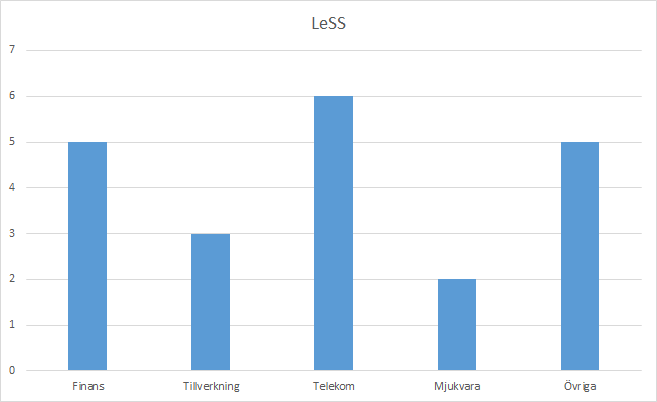
\includegraphics{Grafer/LeSS_brancher.png}
			\end{center}
		
			LeSS har en tyngdunkt som ligger på finans och telekombranschen. Annars är det mjukvaruföretag och tillverkningsföretag som står ur mängden.\\		
				
				
			\title{Scaled Agile Framework branscher}
			\begin{center}
				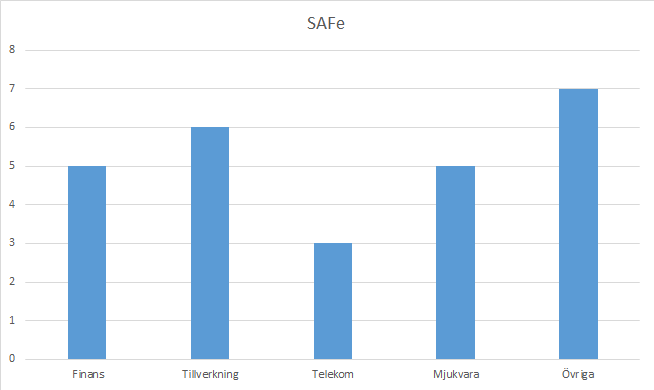
\includegraphics{Grafer/SAFe_brancher.png}
			\end{center}
					
			SAFe har lika som LeSS finansbranschen i toppen, men skiljer sig i och med att både tillverkningsföretag och mjukvaruföretag stiger över telekom.
			
		\subsubsection{Branscher - Slutsatser}
		
			Finansbranschen är återkommande för de båda stora ramverken. Inom finans finns det ovanligt höga krav på säkerhet och kvalitét när det kommer till datasystem. Dels på grund av den känsliga datan men främst för att de är en vanlig målgrupp för cyber-kriminalitet. Inom finans finns det heller sällan ekonomiska hinder för projekt av tillräcklig storlek för att behöva tillämpa ett ramverk för uppskalning. 
			
			Institutioner för finans, såsom banker, kan således konstateras vara bland de första som haft både behov och resurser att implementera ramverken.
			
			
			-Telekom vs Tillverkning, förklara skillnaden \\
			-Tillverkning mer strukturerat (tänk löpande band) \\
			-Telekom mer utspritt, dynamiskt. Många olika system som ska fungera. \\
						
		%todo diskutera varför skillnaderna uppstår, dvs telekom vs. tillverkning -> färdig struktur (löpande band etc) vs kaos
	

	\subsection{Popularitet och adoption}
	
		Mängden tillgänglit material ger en riktgivande uppfattning om i vilken utsträckning ramverken används. Mer entydig data finns dock för att stöda uppfattningen och för att ge en tydligare bild.
		
		Enligt en rapport baserad på en enkät gjort av Version one är SAFe betydligt mer utbrett jämfört med LeSS och DAD. \cite{version_one_report} \\	
		
		Observera att man i själva enkäten kunde kryssa flera alternativ, därav en totalprocent på mer än hundra:
		
		\begin{center}
			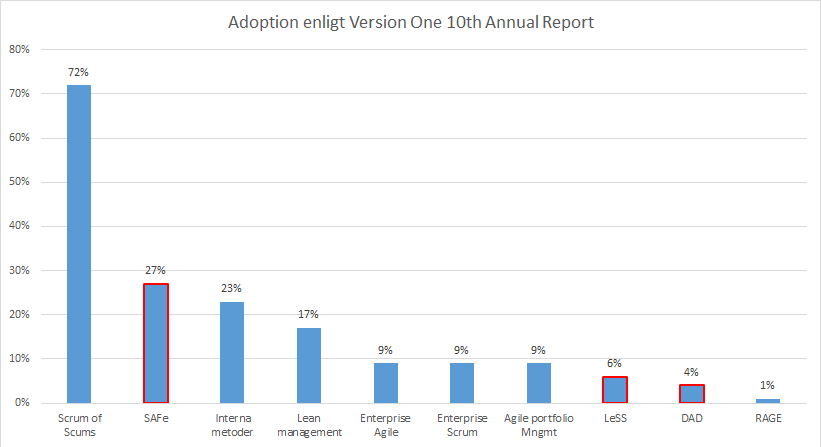
\includegraphics{Grafer/AnnualReport_Adoption.png}
		\end{center}
		\cite{version_one_report}
	
		Den egenskap som korrelar starkast med ett ramverks eller metods popularitet i ovanstående rapport är kostnad. De mest populära ramverken och metoderna i Version One rapporten har även en implementationskostnad listad som 'låg' i Agile Scaling Knowlegde -matrisen. \cite{ask_matrix}				
		Såsom det påpekas i kapitlet om Material och Metoder är många av de populära metoderna inte klassifierbara som ramverk. 
		
		
		Resultatet från enkäten öppnar inte direkt huruvida ramverken är populära jämfört med varandra, förutom att SAfE är i en klass för sig. Sökmotorn Google ger statistik på popularitet av olika över tiden. I egenskap av världens mest populära sökmotor ger denna statistik en god uppfattning om huruvida ett ramverk är allmänt känt och använt eller ej. 
		
		Då alla tre ramverks sökningar sätts emot varandra kan det igen konstateras att det SAFe är klart mer eftersökt. Ur samma data syns DAD och LeSS som lika eftersökta.
		
		Y-axeln är ett automatiskt genererat jämförelsetal direkt korrelerande med antal sökningar per tidsenhet.
		\begin{center}
			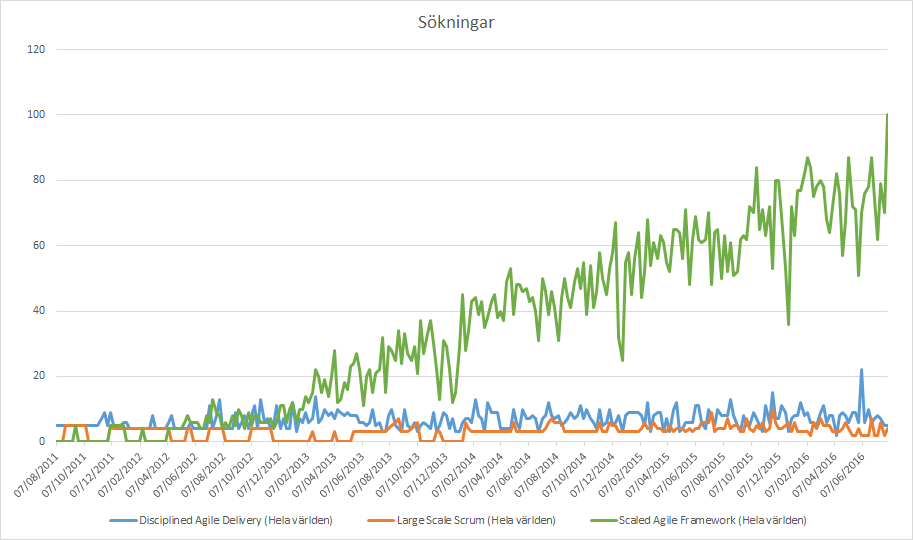
\includegraphics{Grafer/Google_sokningar.png}
		\end{center}
		\cite{google_stats}
	
	
		Genom att utesluta SAFe får man ett noggrannare resultat för LeSS och DAD, vilket är mer ändamålsenligt. DAD genomgår en positivare trend, och är i allmänhet mera eftersökt än LeSS. Detta är motstridigt mot det resultat som rapporterades i Version One rapporten. Detta kan tyda på ett mer utvidgat intresse för DAD i framtiden, då trenden för dess popularitet är klart positiv jämfört med LeSS.
	
		Y-axeln är igen ett jämförelsetal som endast är menat för intern jämförelse inom denna graf.
		\begin{center}
			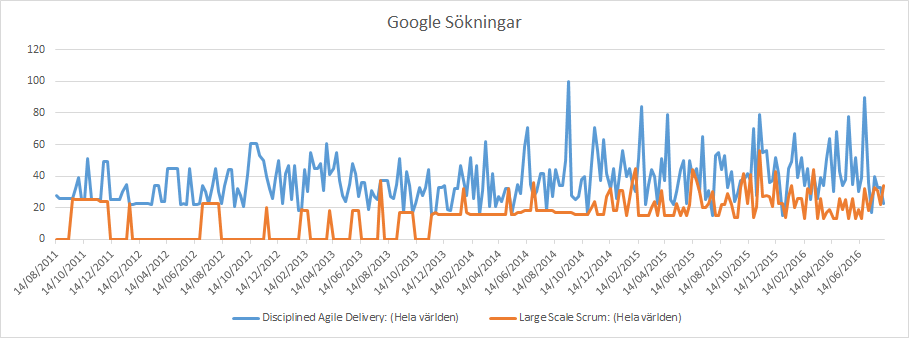
\includegraphics{Grafer/Google_sokningar_dad_less.png}
		\end{center}
		\cite{google_stats_dad_less}
		
		
	\subsection{Jämförelse}
		Ur ASK-matrisen:
		-Kostnader \\
		-Tillgänglig ceritification och skolning
				
				
\section{Diskussion och fortsatt forskning}
	
%\clearpage                     % luku loppuu, loput kelluvat tänne, sivunv.

%\input{luku2}                  % tässä tyylissä ei sivunvaihtoja lukujen
%\input{luku3}                  %   välillä. Toiset ohjaajat haluavat 
%\input{luku4}                  %   sivunvaihdot.

\label{pages:text}
\clearpage                     % luku loppuu, loput kelluvat tänne, sivunvaihto
%\newpage                       % ellei ylempi tehoa, pakota lähdeluettelo 
                               % alkamaan uudelta sivulta

% -------------- Lähdeluettelo / reference list -----------------------
%
% Lähdeluettelo alkaa aina omalta sivultaan; pakota lähteet alkamaan
% joko \clearpage tai \newpage
%
%
% Muista, että saat kirjallisuusluettelon vasta
%  kun olet kääntänyt ja kaulinnut "latex, bibtex, latex, latex"
%  (ellet käytä Makefilea ja "make")

% Viitetyylitiedosto aaltosci_t.bst; muokattu HY:n tktl-tyylistä.
\bibliographystyle{aaltosci_t}
% Katso myös tämän tiedoston yläosan "preamble" ja siellä \bibpunct.

% Muutetaan otsikko "Kirjallisuutta" -> "Lähteet"
\renewcommand{\refname}{Referenser}  % article-tyyppisen
%\renewcommand{\bibname}{Lähteet}  % jos olisi book, report-tyyppinen

% Lisätään sisällysluetteloon
\addcontentsline{toc}{section}{\refname}  % article
%\addcontentsline{toc}{chapter}{\bibname}  % book, report

% Määritä kaikki bib-tiedostot
\bibliography{lahteet}
%\bibliography{thesis_sources,ietf_sources}

\label{pages:refs}
\clearpage         % erotetaan mahd. liitteet alkamaan uudelta sivulta

% -------------- Liitteet / Appendices --------------------------------
%
% Liitteitä ei yleensä tarvita. Kommentoi tällöin seuraavat
% rivit.

% Tiivistelmässä joskus matemaattisen kaavan tarkempi johtaminen, 
% haastattelurunko, kyselypohja, ylimääräisiä kuvia, lyhyitä 
% ohjelmakoodeja tai datatiedostoja.

%\appendix
%\section{Esimerkkiliite}
\label{sec:app1}

Jos työhön kuuluu suurikokoisia (yli puoli sivua) kuvia, taulukoita
tai karttoja tms., jotka eivät kokonsa puolesta sovi tekstin joukkoon,
ne laitetaan liitteisiin. Liitteet numeroidaan. Jokaiseen liitteeseen
tulee viitata tekstissä, eikä liitteisiin ole tarkoitus laittaa ``mitä
tahansa'', vaan vain työlle oikeasti tarpeellista
materiaalia. Liitteisiin voidaan sijoittaa esim. malli
kyselylomakkeesta, jolla tutkimushaastattelu toteutettiin,
pohjapiirustuksia, taulukoita, kaavioita, kuvia tms.

\textbf{TIK.kand suositus: Vältä liitteitä.} Jos iso kuva, mieti onko
sen koko pienettävissä (täytyy olla tulkittavissa) normaalin tekstin
yhteyteen. Joskus liitteeksi lisätään matemaattisen kaavan tarkempi
johtaminen, haastattelurunko, kyselypohja, ylimääräisiä kuvia, lyhyitä
ohjelmakoodeja tai datatiedostoja.

Työtä varten mahdollisesti tehtyjä ohjelmakoodeja ei tyypillisesti
lisätä tänne, ellei siihen ole joku erityinen syy. (Kukaan ei ala
kirjoittaa tai tarkistamaan koko koodia paperilta vaan pyytää sitä
sinulta, jos on kiinnostunut.)

%\subsection{Esimerkkiliitteen otsikko 1}
%\label{sec:app1_1}
%
%Kerätty data-aineisto.
%
% -------------------------------------------------------------- %
%
%\newpage
%\section{Toinen esimerkkiliite}
%\label{sec:app2}
%
%Haastattelukysymykset: mitä, missä, milloin, kuka, miten.



%\label{pages:appendices}

% ---------------------------------------------------------------------

\end{document}
